\chapter{Related Works}

Your related works, and your purpose and contribution which must be different as below.

\section{Mhd Zulfikar Akram Nasution/ 1164081}
\subsection{Teori}
\begin{enumerate}
\item Binary Classification atau diartikan kedalam bahasa indonesia yaitu Klasifikasi Biner adalah tugas dalam mengklarifikasikan elemen-elemen dari himpunan yang diberikan kedalam dua kelompok berdasarkan aturan klarifikasi. Pada ummnya klarifikasi biner akan jatuh ke dalam domain Supervised Learning dan dimana kasus khusus hanya memiliki dua kelas.
\begin{itemize}
\item  Contoh Binary Classification pada gambar 2.1
\end{itemize}
\begin{figure}[ht]
\centering
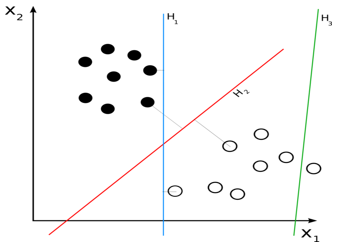
\includegraphics[scale=0.9]{figures/zulfikar/1.png}
\caption{Binary Classification}
\end{figure}

\item Supervised Learning, Unsupervised Learning, dan Clustering
\begin{itemize}
\item Supervised Learning
\end{itemize}
\par
Supervised learning adalah tugas pembelajaran mesin untuk mempelajari suatu fungsi yang memetakan input ke output berdasarkan contoh pasangan input-output. Ini menyimpulkan fungsi dari data pelatihan berlabel yang terdiri dari serangkaian contoh pelatihan. Dalam pembelajaran yang diawasi, setiap contoh adalah pasangan yang terdiri dari objek input (biasanya vektor) dan nilai output yang diinginkan (juga disebut sinyal pengawas). Contoh pada gambar 2.2
\begin{figure}[ht]
\centering
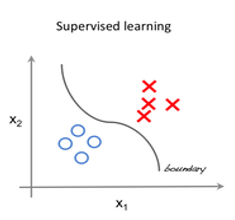
\includegraphics[scale=0.9]{figures/zulfikar/2.png}
\caption{Supervised Learning}
\end{figure}

\begin{itemize}
\item Unsupervised Learning
\end{itemize}
\par
Unsupervised Learning merupakan sebuah data yang belum ditentukan variabelnya jadi hanya berupa data saja. Dalam sebuah kasus Unsupervised Learning adalah aggap saja anda belum pernah membeli buku sama sekali dan pada suatu hari anda telah membeli buku dengan sangat banyak dalam kategori yang berbeda. Sehingga buku tersebut belum di kategorikan dan hanya berupa data buku saja. Coontoh seperti pada gambar 2.3
\begin{figure}[ht]
\centering
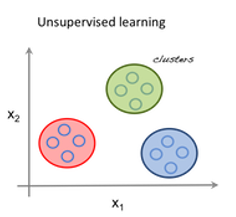
\includegraphics[scale=0.9]{figures/zulfikar/3.png}
\caption{Unsupervised Learning}
\end{figure}

\begin{itemize}
\item Clustering
\end{itemize}
\par
 Classtering merupakan sebuah proses untuk mengklasifikasikan sebuah data dalam satu parameter. Dalam kasus ini dapat dijelaskan ada beberapa orang yang memiliki kekuatan tubuh yang sehat dan kekuatan tubuh yang lemah. Parameter bagi orang yang memiliki tubuh yang kuat adalah orang yang terlihat bugar dan sehat maka dengan orang yang memiliki parameter adalah orang yang memiliki kekuatan tubuh yang kuat dan untuk kekuatan tubuh yang lemah adalah sebaliknya. Contoh seperti pada gambar 2.4
\begin{figure}[ht]
\centering
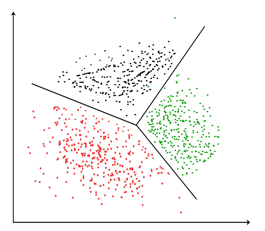
\includegraphics[scale=0.9]{figures/zulfikar/4.png}
\caption{Clustering}
\end{figure}

\item Evaluasi dan Akurasi
\par
 Evaluasi adalah tentang  bagaimana kita dapat mengevaluasi seberapa baik model bekerja dengan mengukur akurasinya. Dan akurasi akan didefinisikan sebagai persentase kasus yang diklasifikasikan dengan benar. Kita dapat menganalisis kesalahan yang dibuat oleh model, atau tingkat kebingungannya, menggunakan matriks kebingungan. Matriks kebingungan mengacu pada kebingungan dalam model, tetapi matriks kebingungan ini bisa menjadi sedikit sulit untuk dipahami ketika mereka menjadi sangat besar.

\item Cara Membuat dan Membaca Confusion Matrix
\begin{itemize}
\item Tentukan pokok permasalahan dan atributnya
\item Buat Decicion Tree
\item Buat Data Testing
\item Mencari nilai variabelnya misal a,b,c, dan d
\item Mencari nilai recall, percision, accuracy, dan error rate
\end{itemize}
\par contoh confusion matrix
	\begin{verbatim}
		Recall = 3/(1+3) = 0,75
		Percision = 3/(1+3 = 0,75
		Accuracy = (5+3)/(5+1+1+3) = 0,8
		Error Rate = (1+1)/(5+1+1+3) 0,2
	\end{verbatim}

\item Cara Kerja K-Fold Cross Validation
	\begin{itemize}
		\item Total instance dibagi menjadi N bagian.
		\item Fold yang pertama adalah bagian pertama menjadii testing data dan sisanya menjadi training data.
		\item Hitung akurasi berdasarkan porsi data tersebut dengan menggunakan persamaan.
		\item Fold yang ke dua adalah bagian ke dua menjadi testing data dan sisanya training data. 
		\item Hitung akurasi berdasarkan porsi data tersebut.
		\item Lakukan step secara berulang hingga habis mencapai fold ke-K.
		\item Terakhir hitung rata-rata akurasi K buah.
	\end{itemize}
\par
Berikut ilustrasi K-Fold Cross Validation seperti pada gambar 2.5
\begin{figure}[ht]
\centering
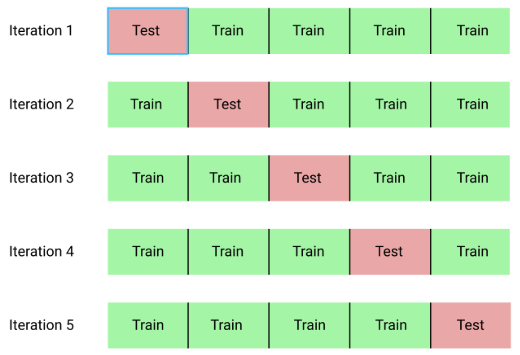
\includegraphics[scale=0.9]{figures/zulfikar/5.png}
\caption{K-Fold Cross Validation}
\end{figure}

\item Decision Tree
\par 
Decision Tree adalah sebuah metode pembelajaran yang digunakan untuk melakukan klarifikasi dan regresi. Decision Tree digunakan untuk membuat sebuah model yang dapat memprediksi sebuah nilai variabel target dengan cara mempelajari aturan keputusan dari fitur data. Contohnya seperti pada gambar 2.6 
\begin{figure}[ht]
\centering
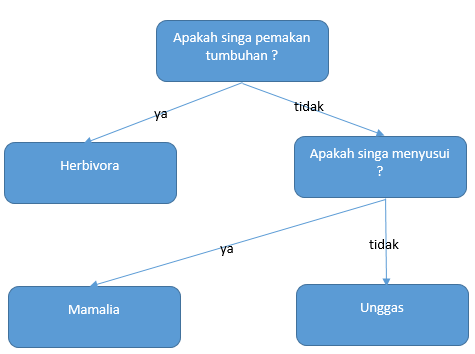
\includegraphics[scale=0.9]{figures/zulfikar/6.png}
\caption{Decision Tree}
\end{figure}

\item Gain dan Entropi
\begin{itemize}
\item Gain adalah pengurangan yang diharapkan dalam enthropy. Dalam mechine learning, gain dapat digunakan untuk menentukan sebuah urutan atribut atau memperkecil atribut yang telah dipilih. Urutan ini akan membentuk decision tree. atribut gain dipilih yang paling besar.
\item  Entropi adalah ukuran ketidakpastian sebuah variabel acak sehingga dapat di artikan entropi adalah ukuran ketidakpastian dari sebuah atribut.
\end{itemize}
\par Contoh seperti pada gambar 2.7
\begin{figure}[ht]
\centering
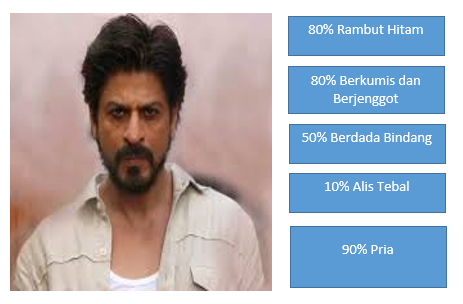
\includegraphics[scale=0.9]{figures/zulfikar/7.png}
\caption{Gain dan Entropi}
\end{figure}
\end{enumerate}

\section{Mhd Zulfikar Akram Nasution/ 1164081}
\subsection{Scikit-Learn}

\begin{enumerate}
\item
\begin{verbatim}
	# load dataset (student mat pakenya)
	import pandas as pd
	lontong    = pd.read_csv('student-mat.csv', sep=';')
	len(lontong)
\end{verbatim}
\begin{figure}[ht]
\centering
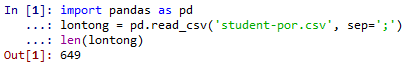
\includegraphics[scale=0.9]{figures/lontong/1.png}
\caption{Load Dataset}
\end{figure}
\par
	Codingan pertama ini akan meload ( menampilkan ) data pada file yang ditentukan. Untuk codingan ini file yang dieksekusi ialah " student-mat.csv " . Secara jelasnya, dalam codingan dapat dilihat bahwa variabel lontong didefinisikan untuk pembacaan csv dari " lontong " dimana untuk pemisahnya yaitu separation berupa ; . Setelah itu variabel lontong di "print" dengan perintah menampilkan "len" panjang ataupun jumlah dan hasilnya berupa angka 649 . 

\item
\begin{verbatim}
	# generate binary label (pass/fail) based on G1+G2+G3 
	# (test grades, each 0-20 pts); threshold for passing is sum>=30
	lontong['pass'] = lontong.apply(lambda row: 1 if (row['G1']+row['G2']+row['G3']) 
											>= 35 else 0, axis=1)
	lontong = lontong.drop(['G1', 'G2', 'G3'], axis=1)
	lontong.head()
\end{verbatim}
\begin{figure}[ht]
\centering
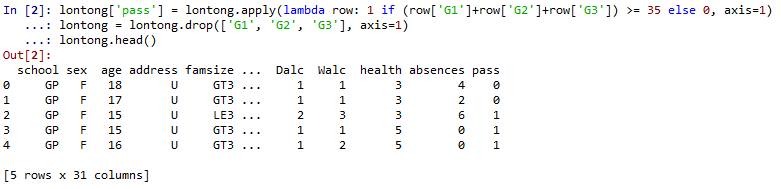
\includegraphics[scale=0.6]{figures/lontong/2.png}
\caption{Generate Binary Label}
\end{figure}
\par
	Codingan kedua ini secara keseluruhan menampilkan  baris  G1, G2 dan G3 ( berdasarkan kriterianya ) untuk kolom PASS pada variabel lontong. Untuk lebih jelasnya, pada codingan terdapat pendefinisian pembacaan "lambda" ( panjang gelombang ) dari baris G1, G2 dan G3. Apabila row-row tersebut bernilai lebih dari 35 maka akan terdefinisikan angka "1" apabila tidak, maka akan terdefinisikan angka "0" pada kolom PASS ( sesuai permintaan awal ). Selanjutnya variabelnya di "print" sehingga menampilkan keluaran. Tidak lupa terdapat juga jumlah dari baris dan kolom yang terubah sesuai dengan baris yang dieksekusi.


\item
\begin{verbatim}
	# use one-hot encoding on categorical columns
	lontong = pd.get_dummies(lontong, columns=['sex', 'school', 'address', 
									'famsize', 
									'Pstatus', 'Mjob', 'Fjob', 
	                               'reason', 'guardian', 'schoolsup', 
								   'famsup', 'paid', 'activities',
	                               'nursery', 'higher', 'internet', 
									'romantic'])
	lontong.head()
\end{verbatim}
\begin{figure}[ht]
\centering
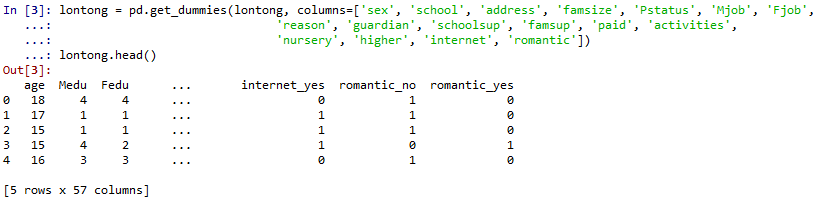
\includegraphics[scale=0.6]{figures/lontong/3.png}
\caption{Pemanggilan get dummies dari lontong}
\end{figure}
\par
	Secara keseluruhan, codingan ini mendefinisikan pemanggilan get dummies ke dalam variabel lontong. Di dalam get dummies sendiri akan terdefinisikan variabel lontong dengan kolom-kolom yang akan dieksekusi seperti school, address dll. Kemudian variabel tersebut di definisikan untuk mendapatkan kembalian berupa keluaran dari eksekusi perintah variabel lontong beserta dengan jumlah baris dan kolom data yang dieksekusi.

\item
\begin{verbatim}
	# shuffle rows
	lontong = lontong.sample(frac=1)
	# split training and testing data
	lontong_train = d[:500]
	lontong_test = d[500:]

	lontong_train_att = lontong_train.drop(['pass'], axis=1)
	lontong_train_pass = lontong_train['pass']

	lontong_test_att = lontong_test.drop(['pass'], axis=1)
	lontong_test_pass = lontong_test['pass']

	lontong_att = lontong.drop(['pass'], axis=1)
	lontong_pass = lontong['pass']

	# number of passing students in whole dataset:
	import numpy as np
	print("Passing: %d out of %d (%.2f%%)" % (np.sum(lontong_pass), len(lontong_pass), 
	       100*float(np.sum(lontong_pass)) / len(lontong_pass)))
\end{verbatim}
\begin{figure}[ht]
\centering
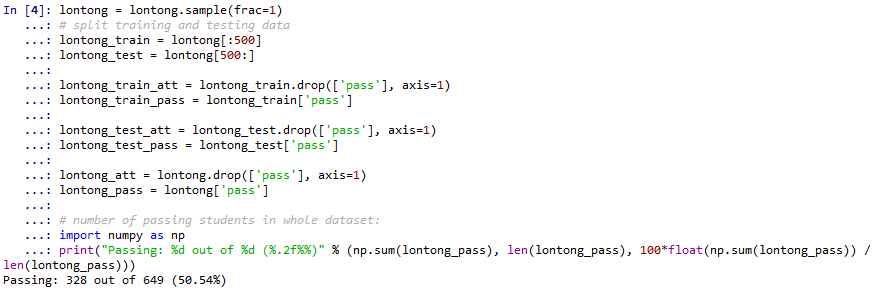
\includegraphics[scale=0.6]{figures/lontong/4.png}
\caption{Mendefinisikan pembagian data}
\end{figure}
\par
	Secara keseluruhan codingan ini difungsikan untuk mendefinisikan pembagian data yang berupa training dan testing data. Secara jelasnya pertama-tama variabel lontong akan mendefinisikan sampel yang akan digunakan ( berupa shuffle row ) . Nah kemudian masing2 parameter yaitu lontong train dan lontong test akan berjumlah 500 data ( telah dibagi untuk training dan testing ). Selanjutnya dilakukan pengeksekusian untuk kolom Pass, apabila sesuai dengan "axis=1" maka eksekusi fungsi berhasil. Selain itu juga disertakan jumlah dari peserta yang lolos dari semua nilai data setnya.

\item 
\begin{verbatim}
	# fit a decision tree
	from sklearn import tree
	soto = tree.DecisionTreeClassifier(criterion="entropy", max_depth=5)
	soto = soto.fit(lontong_train_att, lontong_train_pass)
\end{verbatim}
\begin{figure}[ht]
\centering
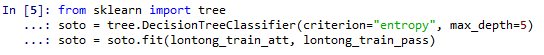
\includegraphics[scale=0.9]{figures/lontong/5.png}
\caption{Membuktikan pengujian}
\end{figure}
\par
	Secara keseluruhan, codingan ini hanya membuktikan pengujian dari Klasifikasi Decision Tree yang ada, apakah true atau tidak dan hasilnya true. Apabila dibahas secara lengkap maka pada codingan ini di definisikan library sklearn untuk mengimpor atau menampilkan tree. Variabel soto difungsikan untuk membaca klasifikasi decision tree dari tree itu sendiri dengan 2 parameternya yaitu kriteria="entropy" dan max depth=5. Maka selanjutnya variabel soto akan masuk dan terbaca dalam module fit dengan 2 parameter yaitu lontong trai att dan lontong train pass.

\item
\begin{verbatim}
	# visualize tree
	import graphviz
	dot_data = tree.export_graphviz(soto, out_file=None, label="all", 
									impurity=False, proportion=True,
	                                feature_names=list(lontong_train_att), 
									class_names=["fail", "pass"], 
	                                filled=True, rounded=True)
	graph = graphviz.Source(dot_data)
	graph
\end{verbatim}
\begin{figure}[ht]
\centering
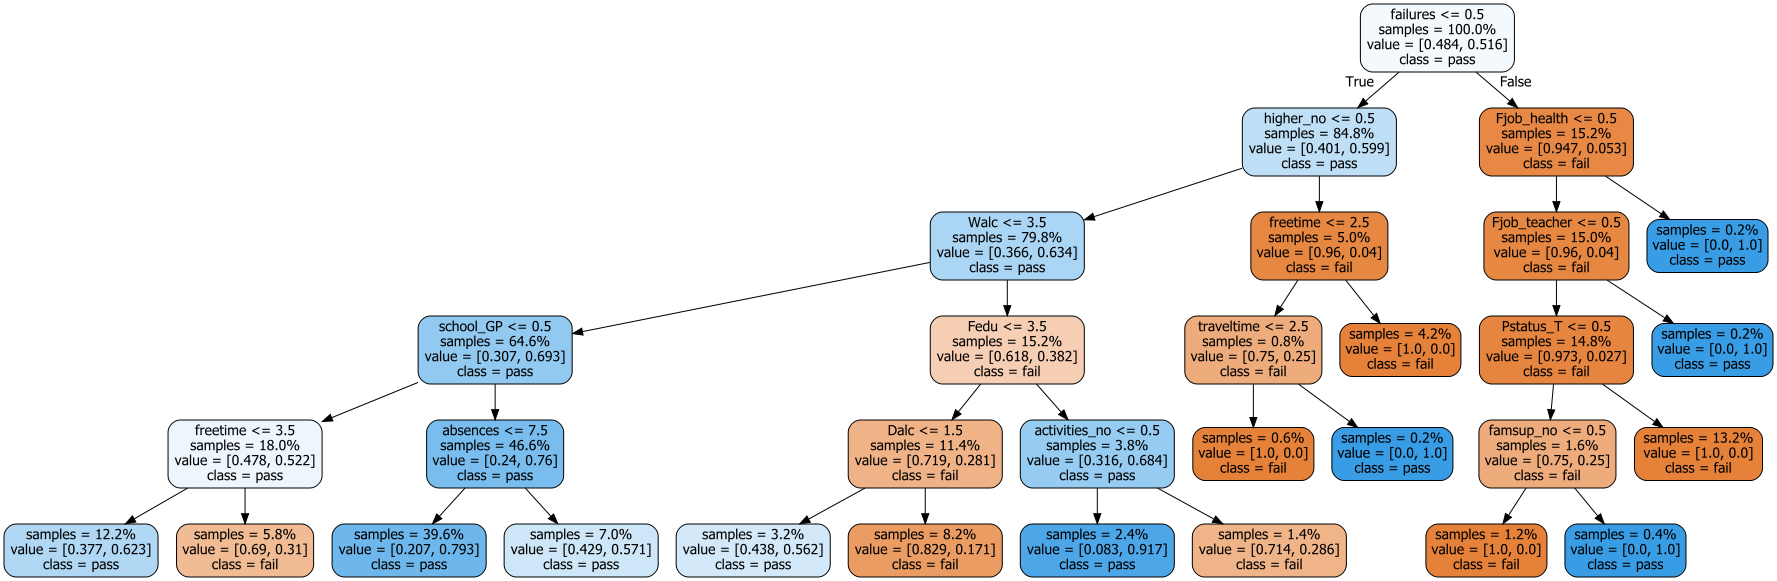
\includegraphics[scale=0.3]{figures/lontong/6.png}
\caption{Gambaran decision tree}
\end{figure}
\par
	Codingan ini memberikan gambaran dari klasifikasi decision tree dari pengolahan parameter yang dieksekusi kedalam variabel soto. Tentunya dengan pemanfaatan library graphviz yang telah diimport dan difungsikan.

\item
\begin{verbatim}
	# save tree
	tree.export_graphviz(soto, out_file="student-performance.dot", 
						 label="all", impurity=False, 
						 proportion=True,
	                     feature_names=list(lontong_train_att), 
	                     class_names=["fail", "pass"], 
	                     filled=True, rounded=True)
\end{verbatim}
\begin{figure}[ht]
\centering
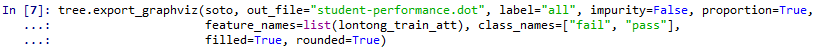
\includegraphics[scale=0.6]{figures/lontong/7.png}
\caption{Library Graphviz}
\end{figure}
\par
	Pada gambar 7 akan menampilkan yang terdapat pada Library Graphviz, apabila benar akan menampilkan hasil output seperti yang terdapat pada gambar.

\item
\begin{verbatim}
	soto.score(lontong_test_att, lontong_test_pass)
\end{verbatim}
\begin{figure}[ht]
\centering
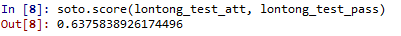
\includegraphics[scale=0.9]{figures/lontong/8.png}
\caption{Menampilkan hasil perhitungan 2 parameter}
\end{figure}
\par
	Menampilkan hasil perhitungan dari kedua parameter yang terdapat pada code tersebut. Yang merupakan perhitungan hasil prediksi silang akan kemungkinan nilai di masa mendatang.

\item
\begin{verbatim}
	from sklearn.model_selection import cross_val_score
	kari = cross_val_score(soto, lontong_att, lontong_pass, cv=5)
	# show average score and +/- two standard deviations away 
	#(covering 95% of scores)
	print("Accuracy: %0.2f (+/- %0.2f)" % (kari.mean(), kari.std() * 2))
\end{verbatim}
\begin{figure}[ht]
\centering
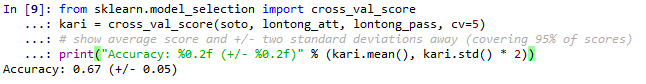
\includegraphics[scale=0.6]{figures/lontong/9.png}
\caption{Mendefinisikan library sklearn}
\end{figure}
\par
	Kodingan tersebut mendefinisikan library sklearn model selection dan import cross val score. Dan kemudian variabel kari mengeksekusi fungsi cross val score(soto, lontong att, lontong pass, cv=5). Kemudian akan menampilkan nilai dari fungsi akurasinya.

\item 
\begin{verbatim}
	for max_depth in range(1, 20):
	    soto = tree.DecisionTreeClassifier(criterion="entropy", 
			max_depth=max_depth)
	    kari = cross_val_score(soto, lontong_att, lontong_pass, cv=5)
	    print("Max depth: %d, Accuracy: %0.2f (+/- %0.2f)" % 
				(max_depth, kari.mean(), kari.std() * 2)
			 )
\end{verbatim}
\begin{figure}[ht]
\centering
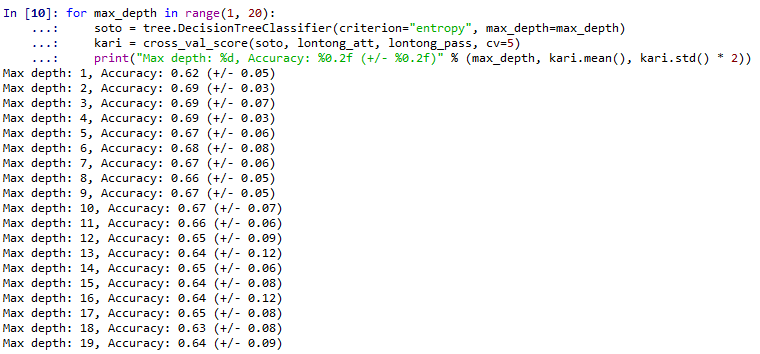
\includegraphics[scale=0.6]{figures/lontong/10.png}
\caption{Menampilkan hasil fungsi max depth dan accuracy}
\end{figure}
\par
	Pada gambar di atas kodingan nya berfungsi untuk menampilkan hasil dari fungsi Max Depth dan Accuraccy dari dari Decission Tree. Yaitu menmpilkan data dari angka 1-20.

\item
\begin{verbatim}
	depth_acc = np.empty((19,3), float)
	i = 0
	for max_depth in range(1, 20):
	    soto = tree.DecisionTreeClassifier(criterion="entropy", 
			max_depth=max_depth)
	    kari = cross_val_score(soto, lontong_att, lontong_pass, cv=5)
	    depth_acc[i,0] = max_depth
	    depth_acc[i,1] = kari.mean()
	    depth_acc[i,2] = kari.std() * 2
	    i += 1

	depth_acc
\end{verbatim}
\begin{figure}[ht]
\centering
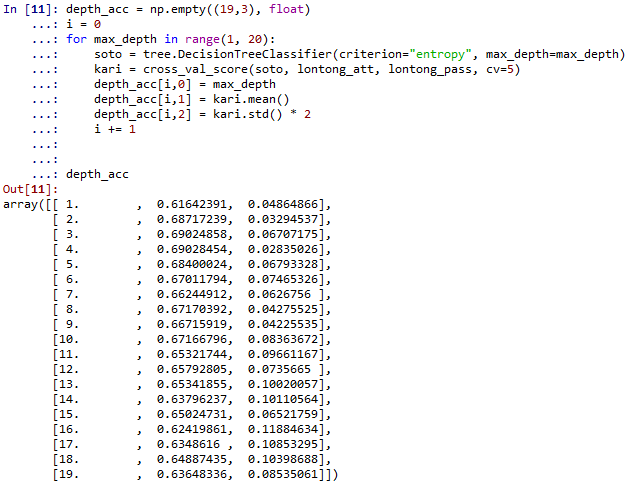
\includegraphics[scale=0.6]{figures/lontong/11.png}
\caption{Menjelaskan variable kari}
\end{figure}
\par
	Dijelaskan bahwa variable kari akan menampilkan atau mendefinisikan nilai dari variabel score yang mana isi dari variable score yaitu soto, lontong att, lontong pass, cv=5. Yang mana hasil tampilan dari kodingannya adalah outputan seperti gambar 11.

\item 
\begin{verbatim}
	import matplotlib.pyplot as plt
	fig, ax = plt.subplots()
	ax.errorbar(depth_acc[:,0], depth_acc[:,1], yerr=depth_acc[:,2])
	plt.show()
\end{verbatim}
\begin{figure}[ht]
\centering
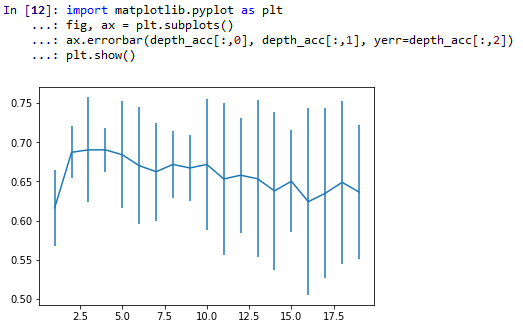
\includegraphics[scale=0.5]{figures/lontong/12.png}
\caption{Menjelaskan dan menampilkan gambar grafik}
\end{figure}
\par
	Pada gambar di atas dijelaskan bahwa pada library matplotlib akan menampilkan gambar grafik pada gambar 12 dari eksekusi fungsi ax.errorbar.

\end{enumerate}


\section{Penanganan Error}
Dari percobaan yang dilakukan di atas, error yang kita dapatkan di dokumentasikan dan di selesaikan(nilai 5 hari kedua):

\begin{enumerate}
	\item
ScreenShoot Error
\begin{figure}[ht]
\centering
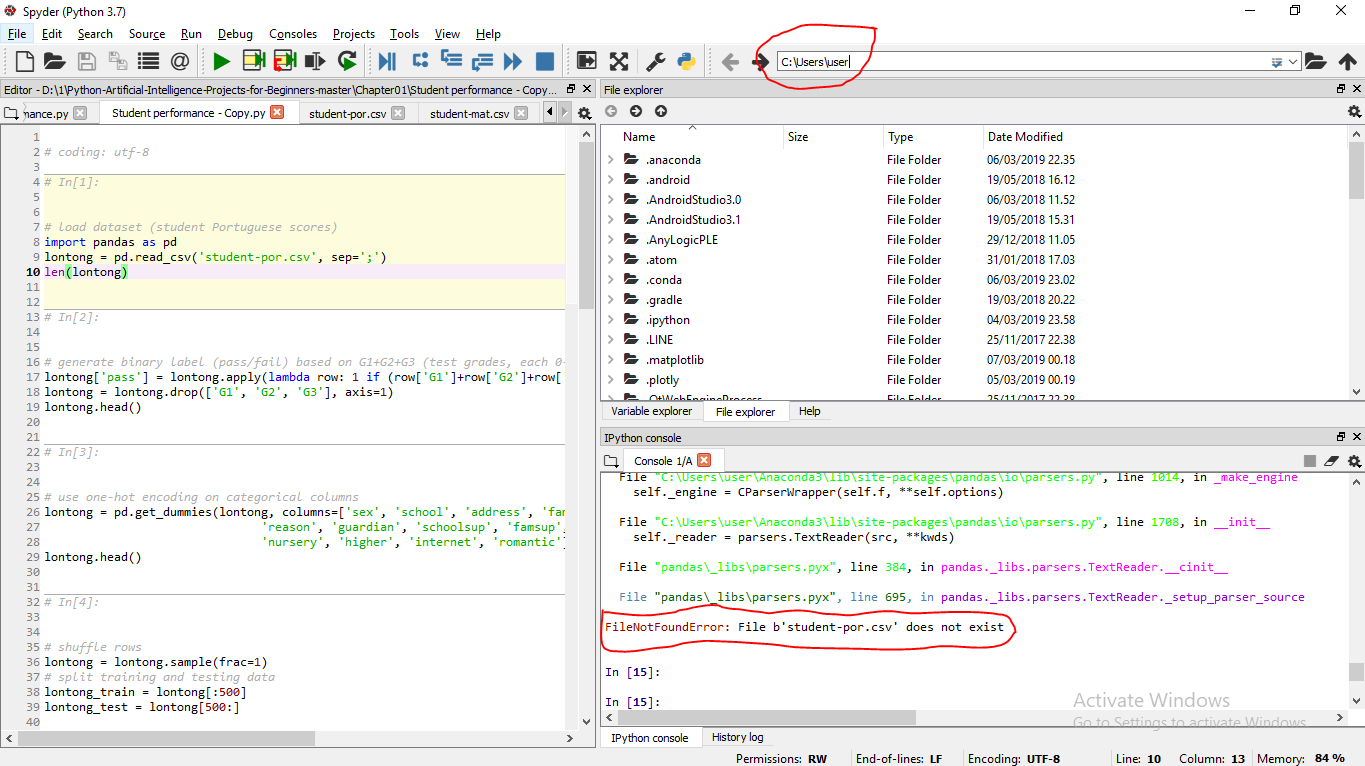
\includegraphics[scale=0.3]{figures/lontong/13.png}
\caption{ScreenShoot Error}
\end{figure}
	\item
Tuliskan kode eror dan jenis errornya
\par
Error ini disebabkan karena pada direktori C tidak terdapat file tersebut. 
	\item
Solusi pemecahan masalah error tersebut
\begin{itemize}
\item 	Masuk ke folder dimana file dataset berada, dapat dilihat dibawah ini
\item 	Setelah diganti, jalankan kembali skrip tersebut pasti akan berhasil
\end{itemize}
\begin{figure}[ht]
\centering
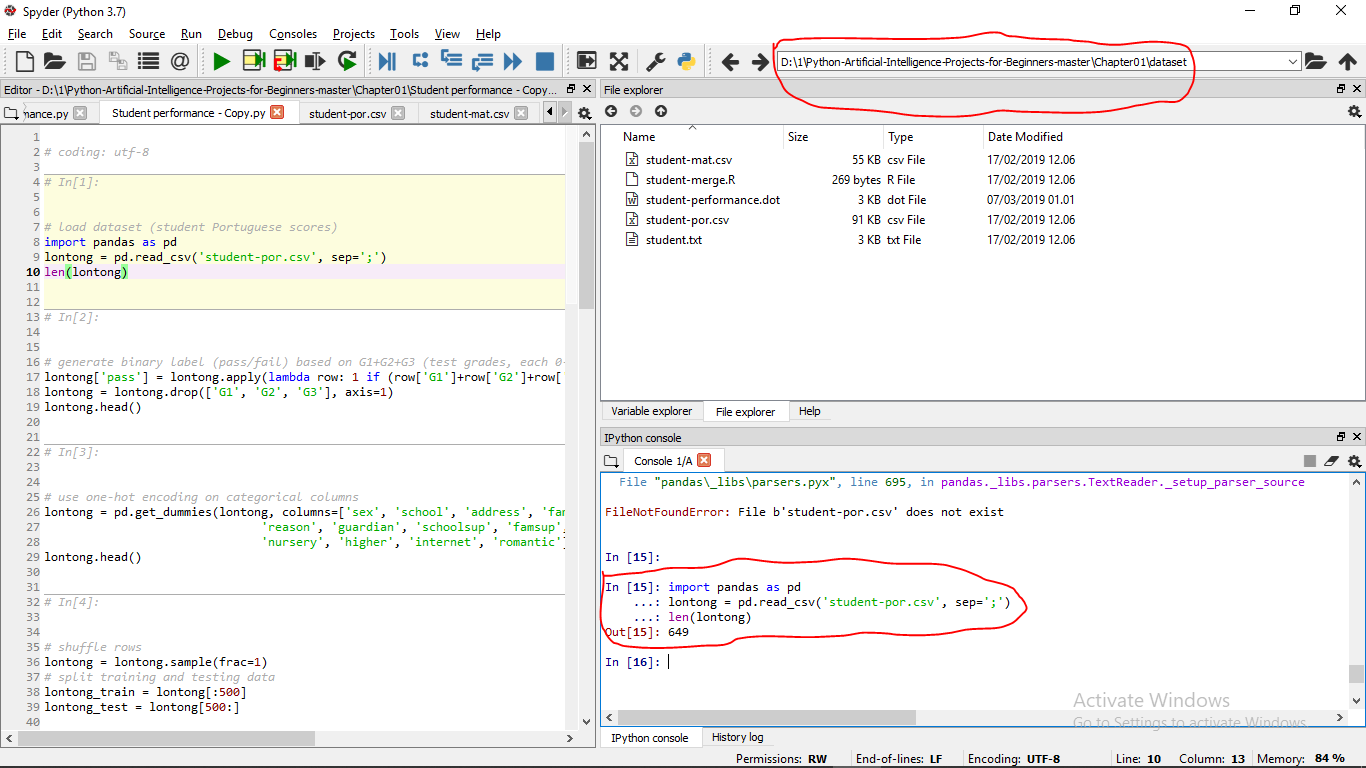
\includegraphics[scale=0.3]{figures/lontong/14.png}
\caption{Penanganan Error}
\end{figure}

\end{enumerate}

\section{Same Topics}
Cite every latest journal with same topic
\subsection{Topic 1}
cite for first topic

\subsection{Topic 2}
if you have two topics you can include here to


\section{Same Method}
write and cite latest journal with same method

\subsection{Method 1}
cite and paraphrase method 1

\subsection{Method 2}
cite and paraphrase method 2 if you have more method please add new subsection.

\section{Teori/Jesron Marudut Hatuan/1164077}
\subsection{Binary classification dilengkapi ilustrasi gambar}
\begin{enumerate}
\item Binary classification yaitu berupa kelas-kelas positif dan kelas-kelas negatif. Klasifikasi biner adalah dikotomisasi yang diterapkan untuk tujuan praktis dan dalam banyak masalah klasifikasi biner praktis, kedua kelompok tidak simetris - daripada akurasi keseluruhan, proporsi relatif dari berbagai jenis kesalahan yang menarik. Misalnya, dalam pengujian medis, false positive (mendeteksi penyakit ketika tidak ada) dianggap berbeda dari false negative atau tidak mendeteksi penyakit ketika hadir.
\begin{figure}[ht]
\centering
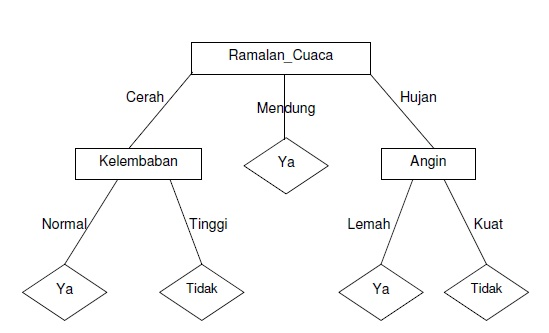
\includegraphics[scale=0.5]{figures/1mrdt.jpg}
\caption{Klasifikasi Binari}
\label{contoh}
\end{figure}
\end{enumerate}


\subsection{ Pengertian Supervised Learning, Unsupervised Learning dan Clustering dan Illustrasi gambar}
\begin{enumerate}
\item Supervised learning adalah sesuatu pembelajaran yang terawasi yang dimana jika output yang diharapkan telah diketahui sebelum-sebelumnya. Biasanya Supervised Learning ini dilakukan dengan menggunakan data yang sudah ada. Pada metode ini, setiap pola yang diberikan kedalam jaringan saraf tiruan setelah diketahui outputnya. Satu pola input akan diberikan ke satu neuron pada lapisan-lapisan input. Pola-pola ini akan dirambatkan di sepanjang jaringan syaraf hingga sampai ke neuron pada lapisan output tersebut. Algoritma pembelajaran yang diawasi menganalisis data pelatihan dan menghasilkan fungsi yang disimpulkan, yang dapat digunakan untuk memetakan contoh-contoh baru. Skenario optimal akan memungkinkan algoritma menentukan label kelas dengan benar untuk instance yang tidak terlihat.
\begin{figure}[ht]
\centering
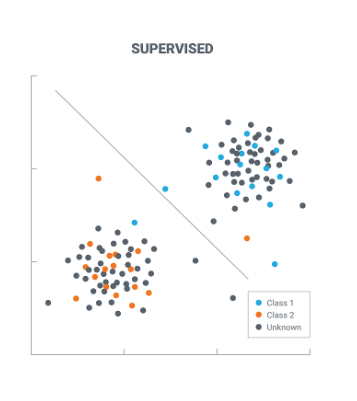
\includegraphics[scale=0.5]{figures/2mrdt.png}
\caption{Supervised Learning}
\label{contoh}
\end{figure}

\item Unsupervised learning merupakan sebuah pembelarajan yang tidak terawasi dimana tidak memerlukan target output. Pada metode ini tidak dapat ditentukan hasil seperti apa yang diharapkan selama proses pembelajaran, nilai bobot yang disusun dalam proses range tertentu tergantung pada sebuah nilai output yang telah diberikan. Tujuan metode unsupervised learning ini agar dapat mengelompokkan unit-unit yang hampir sama dalam satu area tertentu. Pembelajaran ini biasanya sangat cocok untuk klasifikasi pola-pola. Contohny algoritma jaringan saraf tiruan yang menggunakan metode unsupervised ini merupakan competitive, kohonen, LVQ(Learning Vector Quantization), neocognitron.
\begin{figure}[ht]
\centering
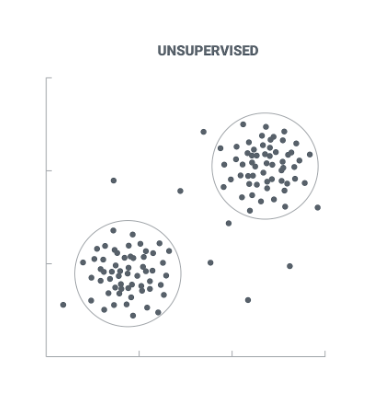
\includegraphics[scale=0.5]{figures/3mrdt.png}
\caption{Unsupervised Learning}
\label{contoh}
\end{figure}
\item Analisis Cluster adalah sebuah teknik statistika yang dapat berguna untuk mengelompokkan sebuah objek-objek ataupun variable-variable ke dalam beberapa grup tertentu dimana pada setiap objek atau variable yang telah terbentuk mempunyai sifat dan karakteristik yang berdekatan tersebut.Gagasan populer mengenai cluster termasuk kelompok dengan jarak kecil antara anggota cluster, area padat ruang data, interval atau distribusi statistik tertentu. Clustering karena itu dapat dirumuskan sebagai masalah optimasi multi-objektif. Algoritma pengelompokan dan pengaturan parameter yang sesuai (termasuk parameter seperti fungsi jarak yang akan digunakan, ambang kepadatan atau jumlah cluster yang diharapkan) tergantung pada set data individual dan penggunaan hasil yang dimaksudkan.
\begin{figure}[ht]
\centering
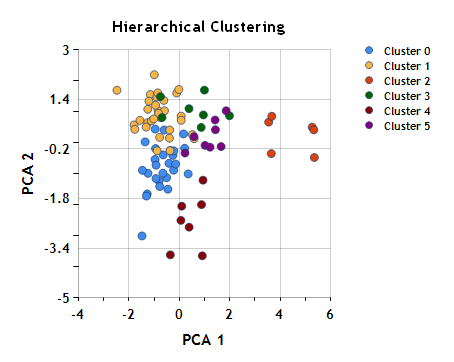
\includegraphics[scale=0.5]{figures/4mrdt.png}
\caption{Cluster}
\label{contoh}
\end{figure}
\end{enumerate}

\subsection{Evaluasi dan akurasi dan Illustrasi gambar}
\begin{enumerate}
\item Evaluasi merupakan suatu langkah bagaimana agar dapat mengevaluasi seberapa baik model bekerja dengan cara mengukur tingkat akurasinya. Dan akurasi tersebut akan didefinisikan menjadi sebuah persentasi studi kasus yang telah diklasifikasikan dengan benar. Dapat juga untuk menganalisis kesalahan yang dibuat oleh sebuah model, atau tingkat kebingungannya, menggunakan matriks kebingungan. Matriks kebingungan mengacu pada sebuah kebingungan dalam model, tetapi matriks kebingungan ini bisa menjadi sedikit sulit untuk dipahami ketika mereka menjadi sangat besar.
\begin{figure}[ht]
\centering
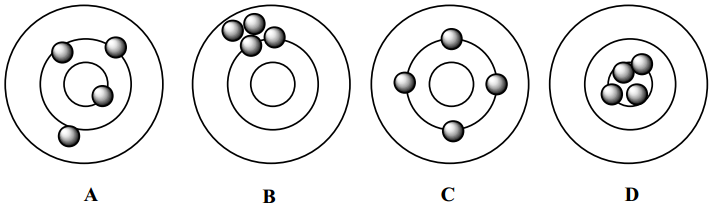
\includegraphics[scale=0.5]{figures/5mrdt.png}
\caption{ Evaluasi dan Akurasi}
\label{contoh}
\end{figure}
\end{enumerate}

\subsection{ Cara membuat dan membaca confusion matrix, buat confusion matrix }
\begin{enumerate}
\item Cara membuat dan membaca confusion matrix :
\begin{itemize}
\item 1)	Menentukan pokok sebuah permasalahan dan atribut-atributnya, misal gaji dan listik.
\item 2)	Buat pohon keputusan
\item 3)	Lalu data testingnya
\item 4)	Lalu mencari nilai a, b, c, dan d. Semisal a = 5, b = 1, c = 1, dan d = 3.
\item 5)	Selanjutnya mencari nilai recall, precision, accuracy, serta dan error rate.
\end{itemize}
\item Berikut adalah contoh dari confusion matrix :
\begin{itemize}
\item Recall =3/(1+3) = 0,75
\item Precision = 3/(1+3) = 0,75
\item Accuracy =(5+3)/(5+1+1+3) = 0,8
\item Error Rate =(1+1)/(5+1+1+3) = 0,2
\end{itemize}
\end{enumerate}

\subsection{Membuat cara K-fold cross validation bekerja dengan gambar ilustrasi}
\begin{enumerate}
\item Cara kerja K-fold cross validation :
\begin{itemize}
\item 1)	Total instance dibagi menjadi N bagian.
\item 2)	Fold yang pertama adalah bagian pertama menjadi data uji (testing data) dan sisanya menjadi training data.
\item 3)	Lalu hitung akurasi berdasarkan porsi data tersebut dengan menggunakan persamaan.
\item 4)	Fold yang ke dua adalah bagian ke dua menjadi data uji (testing data) dan sisanya training data. 
\item 5)	Kemudian hitung akurasi berdasarkan porsi data tersebut.
\item 6)	Dan seterusnya hingga habis mencapai fold ke-K.
\item 7)	Terakhir hitung rata-rata akurasi K buah.
\end{itemize}
\begin{figure}[ht]
\centering
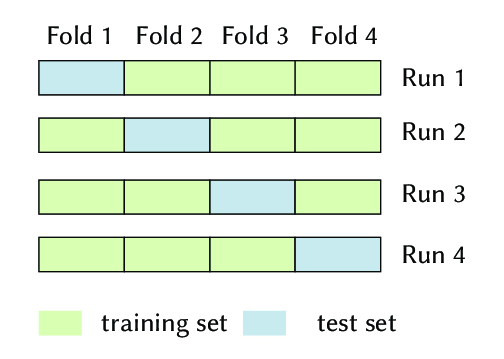
\includegraphics[scale=0.5]{figures/6mrdt.png}
\caption{K-fold cross validation}
\label{contoh}
\end{figure}
\end{enumerate}

\subsection{Decision tree dengan gambar ilustrasi}
\begin{enumerate}
\item Decision Tree dalah metode pembelajaran yang diawasi non-parametrik yang digunakan untuk mengklasifikasi dan regresi. Tujuannya adalah untuk membuat model yang memprediksi nilai variabel target dengan mempelajari aturan keputusan sederhana yang disimpulkan dari fitur data. Decision tree memadukan antara eksplorasi data dan sebuah pemodelan, sehingga sangat bagus sebagai langkah awal dalam proses pemodelan bahkan ketika dijadikan menjadi sebuah model akhir dari beberapa teknik lain.\\
\begin{figure}[ht]
\centering
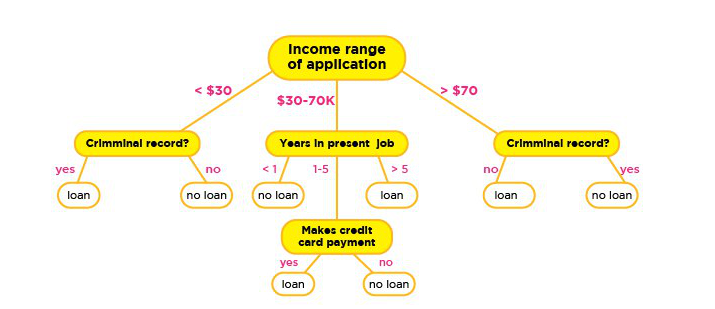
\includegraphics[scale=0.5]{figures/7mrdt.png}
\caption{Decision Tree}
\label{contoh}
\end{figure}
\end{enumerate}

\subsection{Information Gain dan entropi dengan gambar ilustrasi}
\begin{enumerate}
\item Information gain dapat didasarkan kepada penurunan entropi setelah dataset yang sebelumnya dapat dibagi pada atributnya. Untuk membangun sebuah decision tree, merupakan cara agar semua tentang menemukan atribut yang mengembalikan perolehan informasi tertinggi dari yang lainnya.
\begin{figure}[ht]
\centering
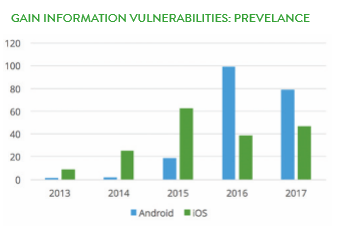
\includegraphics[scale=0.5]{figures/8mrdt.png}
\caption{Information gain}
\label{contoh}
\end{figure}
\item Entropi adalah cara untuk mengukur keacakan dalam sebuah sistem informasi yang sedang diproses. Semakin tinggi entropi, mka hasilnya semakin sulit untuk menarik kesimpulan dari informasi tersebut. Melempar koin merupakan salah satu contoh tindakan yang memberikan informasi yang random. Untuk koin yang tidak memiliki afinitas untuk kepala atau ekor, hasil dari sejumlah lemparan sulit diprediksi. Mengapa? Karena tidak ada hubungan antara membalik dan hasilnya. Inilah inti dari entropi.
\begin{figure}[ht]
\centering
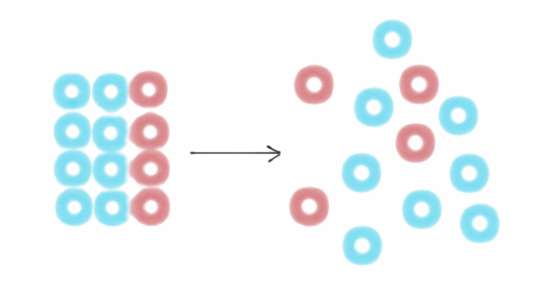
\includegraphics[scale=0.5]{figures/9mrdt.png}
\caption{Entropi}
\label{contoh}
\end{figure}
\end{enumerate}


\subsection{Scikit-learn}
\begin{enumerate}
\item Penjelasan kodingan ini akan menampilkan data pada file yang ditentukan. Untuk codingan ini file yang dieksekusi untuk digunakan ialah student-mat.csv. Dalam codingan dapat dilihat bahwa variabel Rambutan dapat  didefinisikan untuk pembacaan file csv dari  Durian  dimana untuk pemisahnya yaitu separation berupa ; . Setelah itu variabel Rambutan di tampilkan dengan perintah menampilkan len panjang ataupun jumlah dan hasilnya berupa angka 395 . 
\begin{figure}[ht]
\centering
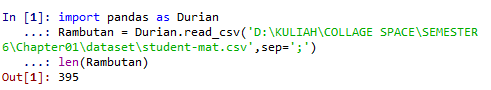
\includegraphics[scale=0.5]{figures/no1.png}
\caption{Load Dataset}
\label{Hasil}
\end{figure}
\end{enumerate}

\begin{enumerate}
\item Kodingan berikut berguna untuk menampilkan setiap baris  G1, G2 dan G3 untuk kolom PASS pada variabel Rambutan. Untuk lebih jelasnya, pada kodingan terdapat pendefinisian pembacaan lamda ( panjang gelombang ) dari baris G1, G2 dan G3. Apabila row-row tersebut bernilai lebih dari 35 maka akan terdefinisikan angka 1 apabila tidak, maka akan terdefinisikan angka 0 pada kolom PASS ( sesuai permintaan awal ). Selanjutnya variabelnya di ditampilkan sehingga menampilkan keluaran. Tidak lupa terdapat juga jumlah dari baris dan kolom yang terubah sesuai dengan baris yang dieksekusi.
\begin{figure}[ht]
\centering
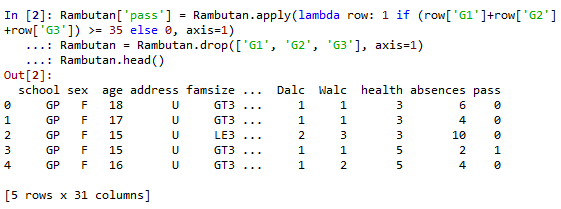
\includegraphics[scale=0.5]{figures/no2.png}
\caption{Generate Binary label}
\label{Hasil}
\end{figure}
\end{enumerate}

\begin{enumerate}
\item Kodingan berikut mendefinisikan pemanggilan get dummies dari Durian dalam variabel Rambutan. Di dalam get dummies sendiri akan terdefinisikan variabel Rambutan dengan kolom-kolom yang akan dieksekusi seperti school, address dll. Kemudian variabel tersebut diartikan untuk mendapatkan kembalian berupa keluaran dari eksekusi perintah variabel Rambutan beserta dengan jumlah baris dan kolom data yang dieksekusi.
\begin{figure}[ht]
\centering
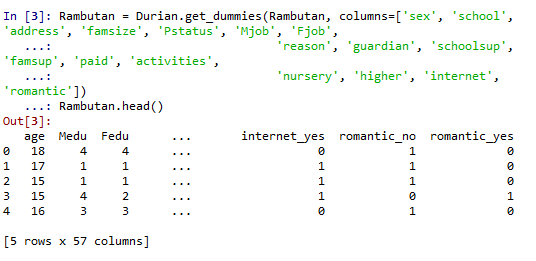
\includegraphics[scale=0.5]{figures/no3.png}
\caption{Use one-hot encoding}
\label{Hasil}
\end{figure}
\end{enumerate}

\begin{enumerate}
\item Kodingan ini dipakai untuk mengartikan pembagian data yang berupa training dan testing data. Pertama-tama variabel Rambutan akan mengartikan sampel yang akan digunakan. Selanjutnya masing-masing parameter yaitu Rambutan train dan Rambutan test akan berjumlah 500 data. Selanjutnya dilakukan pengeksekusian untuk kolom Pass, apabila sesuai dengan axis=1 maka eksekusi fungsi berhasil. Selain itu juga disertakan jumlah dari peserta yang lolos dari semua nilai data setnya.  
\begin{figure}[ht]
\centering
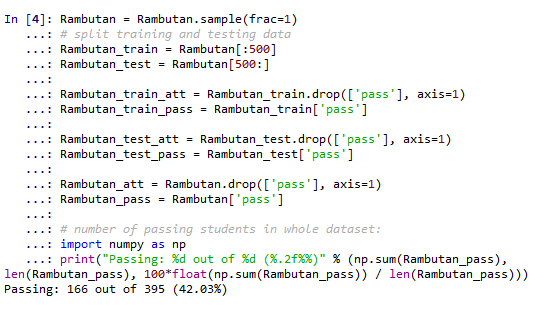
\includegraphics[scale=0.5]{figures/no4.png}
\caption{Shuffle rows}
\label{Hasil}
\end{figure}
\end{enumerate}

\begin{enumerate}
\item Kodingan ini dapat membuktikan pengujian dari Klasifikasi Decision Tree yang ada, apakah true atau tidak dan hasilnya true. Pada kodingan ini di definisikan library sklearn untuk mengimpot atau menampilkan tree. Variabel timun difungsikan untuk membaca klasifikasi decision tree dari tree itu sendiri dengan 2 parameternya yaitu kriteria=entropy dan max depth=5. Maka selanjutnya variabel timun akan masuk dan terbaca dalam module fit dengan 2 parameter yaitu Rambutan trai att dan Rambutan train pass.
\begin{figure}[ht]
\centering
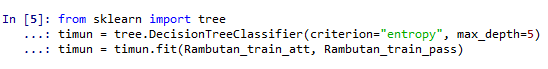
\includegraphics[scale=0.5]{figures/no5.png}
\caption{Fit a Decision tree}
\label{Hasil}
\end{figure}
\end{enumerate}

\begin{enumerate}
\item Penjelasan kodingan ini memberikan gambaran dari klasifikasi decision tree yaitu pengolahan parameter yang dieksekusi kedalam variabel timun. Tentunya dengan pemanfaatan library graphviz yang telah diimport dan difungsikan.
\begin{figure}[ht]
\centering
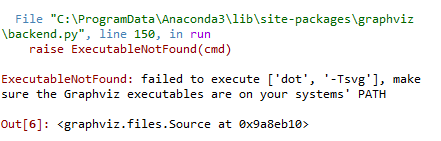
\includegraphics[scale=0.5]{figures/no6.png}
\caption{Visualize tree}
\label{Hasil}
\end{figure}
\end{enumerate}

\begin{enumerate}
\item Penjelasan kodingan ini membahas tentang penyimpanan tree dari library graphviz yang dieksekusi bersamaan dengan variabel timun dan parameter lainnya. Dilakukan pengecekan dan pengujian apakah klasifikasi decision treenya dapat berjalan atau tidak. Apabila tidak berjalan, maka akan terjadi error, namun kodingan ini berfungsi.
\begin{figure}[ht]
\centering
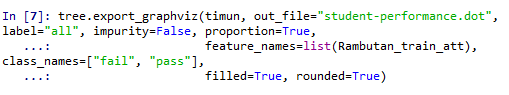
\includegraphics[scale=0.5]{figures/no7.png}
\caption{Save tree}
\label{Hasil}
\end{figure}
\end{enumerate}

\begin{enumerate}
\item Penjelasan kodingan ini membaca skore dari variabel timun dimana terdapat 2 parameter yang dihitung dan diuji yaitu Rambutan test att dan Rambutan test pass. Untuk hasilnya sendiri mengapa berupa angka, dikarenakan pada parameter yang dieksekusi memang memiliki data sehingga dieksekusi dan menghasilkan keluaran dari score tersebut.
\begin{figure}[ht]
\centering
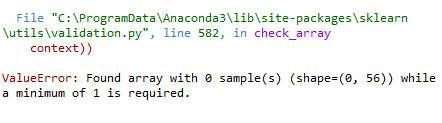
\includegraphics[scale=0.5]{figures/no8.png}
\caption{Score}
\label{Hasil}
\end{figure}
\end{enumerate}

\begin{enumerate}
\item Penjelasan kodingan ini membahas mengenai pengkesekusian fungsi dan variabel dari library yang didefinisikan dan yang diimport. Penjelasan lebih jelasnya ialah kodingan ini mendefinisikan library sklearn.model.selection kemudian mengimport cross val score. Kemudian variabel score mendefinisikan cross val score yang telah diimport tadi dengan 4 parameter yaitu timun, Rambutan att, Rambutan pass dan cv=5 untuk dieksekusi. Setelah semua pemrosesan tersebut maka hasil yang di tampilkan ialah rata-rata perhitungan dari variabel score dimana dan standar dari plus minusnya tentunya dengan ketentuan parameter Accuracy .
\begin{figure}[ht]
\centering
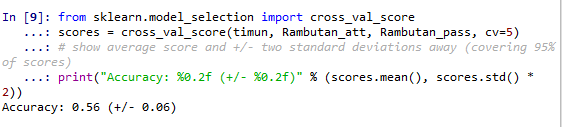
\includegraphics[scale=0.5]{figures/no9.png}
\caption{Show Averange score}
\label{Hasil}
\end{figure}
\end{enumerate}

\begin{enumerate}
\item Penjelasan kodingan ini mendefinisikan max depth dalam jarak angka antara parameter 1 dan 20. Variabel timun mendefinisikan klasifikasi decision tree dengan 2 parameter. Kemudian variabel score mengeksekusi parameter lainnya yaitu seperti timun, Rambutan att, Rambutan pass dan cv=5 ) . Hasil yang ditampilkan ialah dari max depth, accuracy dan plus minusnya dan akhirnya hasil outputannya keluar.
\begin{figure}[ht]
\centering
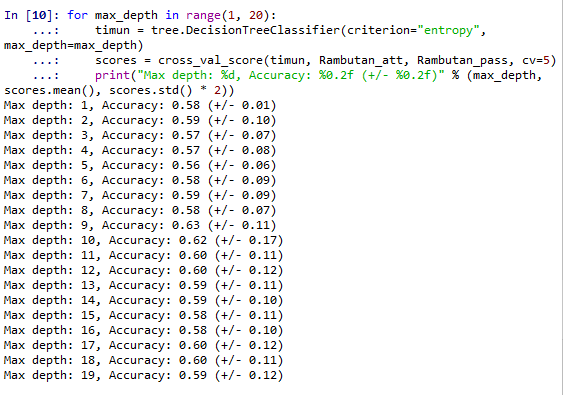
\includegraphics[scale=0.5]{figures/no10.png}
\caption{Max depth}
\label{Hasil}
\end{figure}
\end{enumerate}

\begin{enumerate}
\item Kodingan ini mengartikan bahwa variabel depth\_acc akan mengeksekusi empty dari importan library numphy yang dinamakan np dengan 2 parameter yaitu 19,3 dan float. i didefinisikan dengan angka 0 kemudian untuk perhitungan jarak max depth diantara parameter 1 dan 20. Variabel np mengartikan klasifikasi decision tree dengan 2 parameter. Setelah itu, variabel score mendefinisikan variabel depth\_acc dengan i dan 0, variabel kedua dari depth\_acc dengan i dan 1 serta variabel ketiga dari depth\_acc dengan i dan 2, maka pengeksekusian akhir bahwa variabel i akan ditambah dengan angka 1 untuk hasil akhirnya. Keluarannya akan berupa array dari perhitungan parameter dan variabel yang telah didefinisikan sebelumnya.
\begin{figure}[ht]
\centering
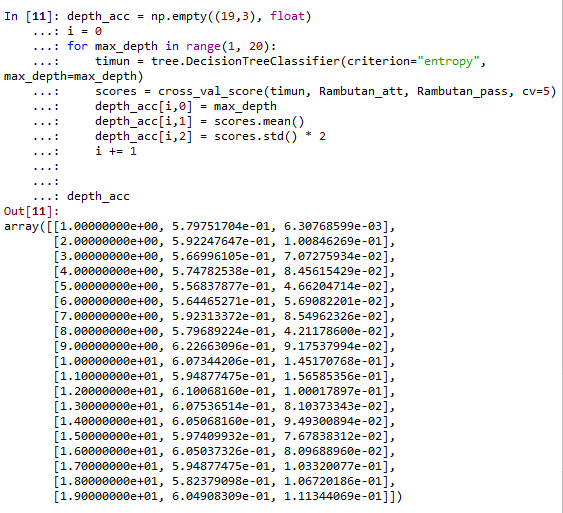
\includegraphics[scale=0.5]{figures/no11.png}
\caption{Depth Acc}
\label{Hasil}
\end{figure}
\end{enumerate}

\begin{enumerate}
\item Kodingan mendefinisikan pemanggilan dari library matplotlib.pyplot sebagai salak sehingga nanti hasilnya akan berbentuk gambar grafik/gelombang. Untuk variabel fig dan ax akan mendefinisikan subplots dari salak. Setelah itu ketentuan dari parameter depth acc = 0, depth acc = 1 dan depth acc 2. Selanjutnya untuk menampilkan gelombang maka panggil variabel salak dengan perintah show.
\begin{figure}[ht]
\centering
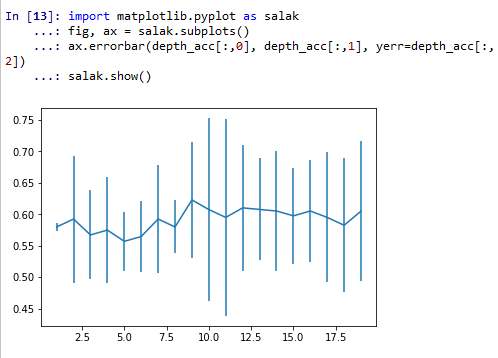
\includegraphics[scale=0.5]{figures/no12.png}
\caption{Import}
\label{Hasil}
\end{figure}
\end{enumerate}

\subsection{Penanganan Eror}
\begin{enumerate}
\item Kodingan eror dan jenis erornya : sebenarnya tidak terdapat eror pada codingan ini namun saat pertama kali di run current cell codingan ini akan eror dan tidak keluar outputannya dikarenakan library graphviz sebelumnya tidak ditemukan atau belum di install terlebih dahulu.
\subitem 
\begin{verbatim}
import graphviz
dot_data = tree.export_graphviz(buahapel, out_file=None, label="all", impurity=False, proportion=True,
                                feature_names=list(buahpir_train_att), class_names=["fail", "pass"], 
                                filled=True, rounded=True)
graph = graphviz.Source(dot_data)
graph
\end{verbatim}
\item Solusi pemecahan masalah eror tersebut yaitu dengan cara menginstall terlebih dahulu library graphviznya pada anaconda prompt atau command prompt dengan perintah conda install graphviz setelah itu run kembali codingan No 8 maka akan muncul outputan atau tampilan keluarannya.
\end{enumerate}

 